\documentclass[10pt]{article}
\usepackage[utf8]{inputenc}
\usepackage{graphicx} % Required for inserting images
\usepackage[english]{babel}
\usepackage{fancyhdr} %  for constructing headers and footers
\usepackage{indentfirst} % indent first paragraph after section header
\usepackage{multicol} % Split on 2 halves
\usepackage{rotating}
\pagestyle{fancy}
\rhead{\thepage}
\graphicspath{ {./top_250_movies.png} }
\graphicspath{ {./comparison.png} }


\begin{document}

\title{\textbf{Comparative Analysis}}
\author{
         {Mussa Shaukenov} \\
         {\small Kazakh-British Technical University} \\ 
         {\small Almaty, 2023}
    }
\date{}

\maketitle

\begin{multicols}{2}
\noindent \footnotesize \textbf{\textit{Abstract} - the work compares the films that were filmed before and after 2000 year according to IMDB top 250 movies dataset.
    }
    
\section*{\centering \normalsize  Introduction}
    \footnotesize{
        Personally, I like to watch movies, especially old ones that were filmed before 2000 year, and do 
        not have so much passion and emotions from modern movies that were filmed after 2000 year. 
        Of course, there are some good movies such as "Interstellar", "Gentlemen" and so on. 
        However, if I had a chance to watch a movie one more time, I would prefer to watch "The Shawshank Redemption" rather than "Avangers".
        Thus, I have decided to make the current work: to make a comparison analysis between
        films shot before 2000 \textbf{(A)} and after 2000 year \textbf{(B)} according to the dataset called "IMDB Top 250 Movies".
    }

\section*{\centering \normalsize  Methods and Tools}
    \footnotesize{
        In the work, I used the Python programming language, and decided to test out the new IDE by JetBrains called DataSpell which is firstly made for data scientists and machine learning engineers.
        It is similar to Jupyter Notebook, and it also uses IPython Notebook. I used the most common combination of libraries in Python that are Pandas and Matplotlib.
    }

\section*{\centering \normalsize  Analysis and Results}
    \footnotesize{
        To start analysis, I filtered CSV file into 2 parts: to movies that were shot before and after 2000 year.
        As a result of filtering data, among 250 movies, 154 movies in the top 250 were produced before the age of 2000, 
        and 96 movies are produced after 2000 year.
        \par Before giving the final result, I wanted to know the flow of ratings, are ratings of modern movies higher or lower compared to movies shot decades ago.
        Therefore, I plotted the following scatter graph to visually display the ratings of movies in Figure 1.
        \begin{center}
            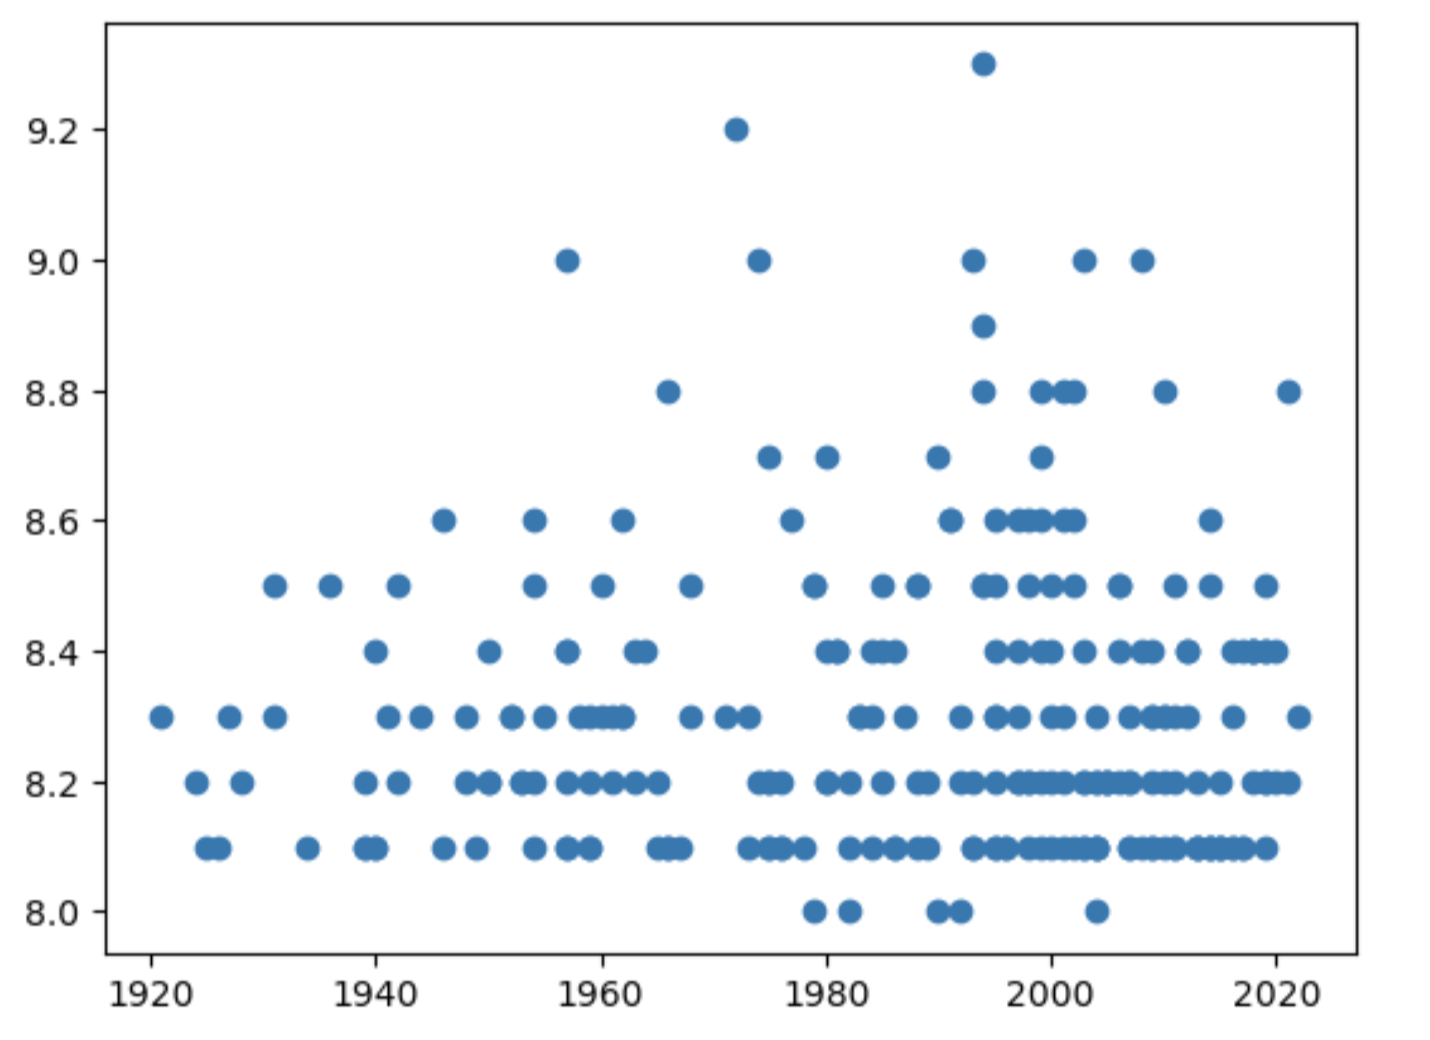
\includegraphics[width=5.5cm, height=4cm]{top_250_movies.png}
            Figure 1. Scatter graph of Top 250 IMDB movies.
        \end{center}

        \par From the graph above, it is apparent that the average ratings of movies are almost the same starting from 1920 year till 2020 year.
        But it is worth mentioning the highest ratings, e.g. higher than 9.0 were shot on the period from about 1980 to 2005 years.
        We can also see that the number of medium movies, e.g. ratings are 8.2 and lower were shot after 2000 year.

        However, from the scatter graph is not understandable how many movies are in the top 250, and which movies present there more: A or B.

        To answer the question, I built pie chart with percentage comparison between A and B movies.
        
        \begin{center}
            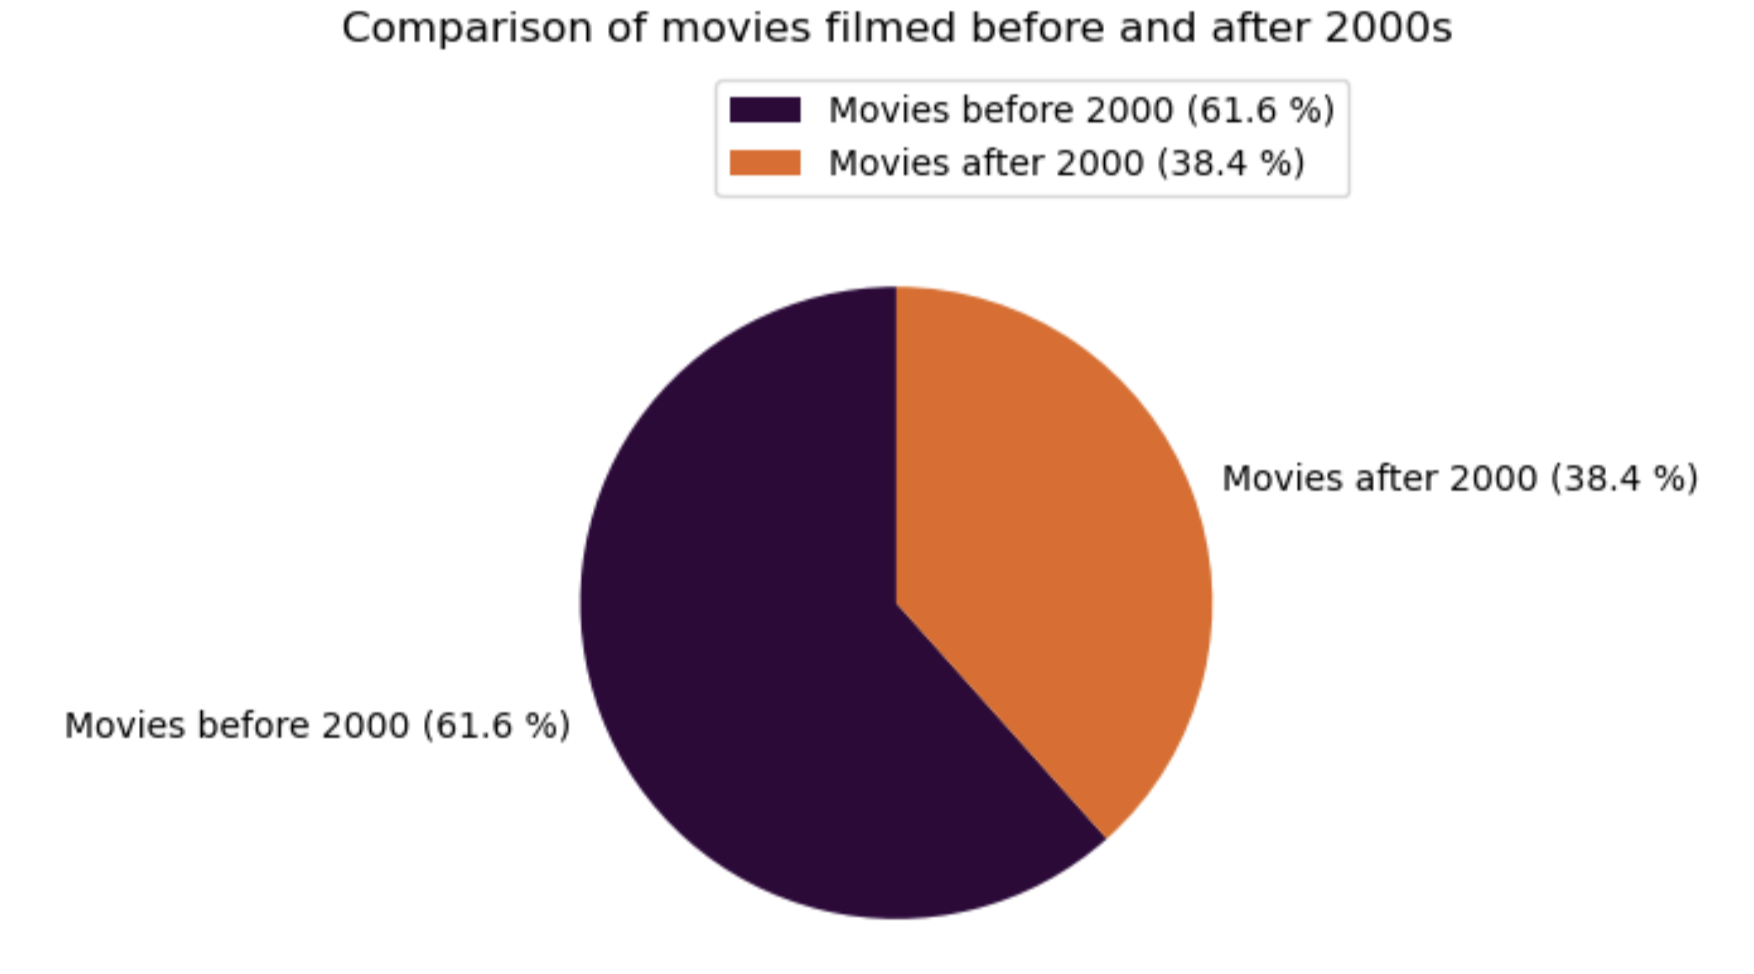
\includegraphics[width=5.5cm, height=3cm]{comparison.png}
            Figure 2. Pie chart with comparison of A and B movies.
        \end{center}
    }

\section*{\centering \normalsize  Conclusion}
    \footnotesize{
        From Figure 2, we can see that almost two halves of the best 250 movies according to IMDB were produced before the age of 2000,
        and it is understandable because there are a lot of great old movies such as "Terminator", "Godfather", etc. 
        So I can safely say that I am not the only one who likes old movies, but also 60\% of IMDB viewers.
        \par P.S. Chances are that if you watch too many movies before 2000 year, you won't be able to watch modern movies from start to finish.

    }

\section*{\centering \normalsize  References}
    \footnotesize{
        \begin{enumerate}
                \item Dataset -- IMDB Top 250 Movies.
                \item Source code -- GitHub Mussa Shaukenov
                \item DataSpell JetBrains
        \end{enumerate}
    }



\end{multicols}


\end{document}